\documentclass[11pt]{article}
\usepackage[a4paper,margin=27mm]{geometry}
\usepackage[T1]{fontenc}
\usepackage{lmodern}
\usepackage{amsmath,amssymb,amsthm,mathtools}
\usepackage{microtype}
\usepackage{tikz}
\usepackage[numbers,sort&compress]{natbib}
\usepackage[hidelinks]{hyperref}
\usepackage{enumitem}
\setlist{nosep}
\hypersetup{pdftitle={Arbitrarily clustered hot spots on bridgeless quantum graphs},
  pdfauthor={Xiaojian Zeng}}
\numberwithin{equation}{section}
\newtheorem{theorem}{Theorem}
\newtheorem{lemma}{Lemma}
\theoremstyle{remark}
\newtheorem{remark}{Remark}
\newcommand{\diam}{\operatorname{diam}}
\newcommand{\dist}{\operatorname{dist}}
\newcommand{\dd}{\,\mathrm{d}}
\newcommand{\M}{\mathcal M}
\newcommand{\T}{T_m}
\newcommand{\G}{\Gamma_m}
\newcommand{\Hstd}{H_{\mathrm{std}}}
\newcommand{\HDD}{H_{\mathrm{DD}}}
\DeclareMathOperator{\argmax}{arg\,max}
\DeclareMathOperator{\argmin}{arg\,min}

\title{Arbitrarily clustered hot spots on bridgeless quantum graphs}
\author{Xiaojian Zeng\thanks{Email: \href{mailto:xiaojianzeng@foxmail.com}{xiaojianzeng@foxmail.com}.}\\
  \small PBC School of Finance, Tsinghua University, 100190}
\date{}

\begin{document}
\maketitle

\begin{abstract}
We construct finite compact metric multigraphs with standard Kirchhoff
conditions, diameter one, and a simple first positive Laplacian eigenvalue,
whose complete set of global maxima and minima has arbitrarily small
diameter. Every edge belongs to a cycle. This proves Conjecture~8.9 of
Kennedy and Rohleder on the hot spots of quantum graphs in its stated
no-bridge sense. The construction combines an explicit specialization of
their split-tree family with the known operation of uniformly doubling
edges. For an integer \(m\geq4\), the first positive eigenvalue is
\(\bigl[\arctan((2m+1)^{-1/2})/h_m\bigr]^2\), where
\(h_m=\pi^{-1}\arctan(m^{-1/2})\), and the complete extrema set has
diameter \(6h_m\). We prove the ordering and simplicity in the full
operator domain and control distances between interior points of the
doubled edges. The result concerns homogeneous network diffusion;
articulation vertices and growing total length and degree are allowed.
\end{abstract}

\noindent\textbf{Keywords:} metric graphs; Kirchhoff Laplacian; hot spots;
network diffusion; spectral geometry.

\section{The hot-spot distance question}

Let \(\Gamma\) be a finite connected compact metric multigraph.
Its edges are intervals of strictly positive finite lengths,
and \(H_\Gamma\) acts as \(-\mathrm{d}^2/\mathrm{d}x^2\).
The domain consists of edgewise \(H^2\) functions that are continuous
at each vertex and satisfy
\begin{equation}\label{eq:kirchhoff}
  \sum_{e\sim v}\partial_{\nu_e}f(v)=0.
\end{equation}
Here \(\partial_{\nu_e}\) points from the vertex into the incident edge.
At a vertex of degree one this is a Neumann condition.
The Hilbert space is the unweighted space
\(L^2(\Gamma)=\bigoplus_e L^2(0,L_e)\).
The associated energy form is
\[
  q_\Gamma(f)=\sum_e\int_0^{L_e}|f'_e(x)|^2\dd x
\]
on continuous edgewise \(H^1\) functions. Thus the spectrum is discrete,
\(0=\mu_1(\Gamma)<\mu_2(\Gamma)\leq\mu_3(\Gamma)\leq\cdots\),
with a simple constant zero mode.

When \(\mu_2(\Gamma)\) is simple, take any nonzero real eigenfunction
\(\psi_2\) and define
\begin{equation}\label{eq:extrema}
  \M(\Gamma)=\argmax_\Gamma\psi_2\;\cup\;\argmin_\Gamma\psi_2.
\end{equation}
This set is unchanged by rescaling or reversing the sign of \(\psi_2\).
Both extrema are global over the whole metric graph, including edge
interiors and all ties. All distances below are shortest-path distances
within the graph.

Kennedy and Rohleder proved that \(\diam\M/\diam\Gamma\) can be
arbitrarily small on trees
\cite[Proposition~4.11 and Example~6.2]{KennedyRohleder2021}.
Their Conjecture~8.9 asks for the same conclusion on doubly connected
metric graphs. Their definition in Section~4.2 means that every point
lies on a cycle; for the finite connected multigraphs considered here
this is the absence of bridges. It permits articulation vertices.
The following explicit construction establishes that conjecture.

\begin{theorem}\label{thm:main}
For every \(\varepsilon>0\) there exists a finite connected compact
standard-Kirchhoff metric multigraph \(\Gamma\) such that every edge
lies on a cycle,
\[
  \diam\Gamma=1,\qquad
  \dim\ker(H_\Gamma-\mu_2(\Gamma))=1,\qquad
  \diam\M(\Gamma)<\varepsilon.
\]
More precisely, for each integer \(m\geq4\), set
\begin{equation}\label{eq:parameters}
  h_m=\frac{\arctan(m^{-1/2})}{\pi},\qquad
  \theta_m=\arctan((2m+1)^{-1/2}),\qquad
  k_m=\frac{\theta_m}{h_m}.
\end{equation}
There is a graph \(\Gamma_m\) for which
\begin{equation}\label{eq:main-formulas}
  \mu_2(\Gamma_m)=k_m^2<\pi^2,\qquad
  \diam\Gamma_m=1,\qquad
  \diam\M(\Gamma_m)=6h_m,
\end{equation}
and \(\M(\Gamma_m)\) consists of exactly \(2m\) vertices.
The choice
\begin{equation}\label{eq:epsilon-choice}
  m=\max\left\{4,\left\lceil\frac{36}{\pi^2\varepsilon^2}\right\rceil\right\}
\end{equation}
gives the required strict inequality.
\end{theorem}

Our comparison tree is a specialization of the published split-tree
construction \cite[Example~6.2]{KennedyRohleder2021}. Uniform replacement
of every edge by two equal-length parallel edges is an established
operation, discussed in \cite[Section~4.3]{Kennedy2024}.
The contribution here is the explicit no-bridge consequence, with full
spectral ordering, the complete extrema set, and the continuum metric
diameter proved below. We make no claim of a new doubling method or
exhaustive historical priority. A bounded primary-literature check
through October 2026 identified no earlier equivalent resolution.

\section{An explicit comparison tree}

Fix \(m\geq4\), abbreviate \(h=h_m\), \(\theta=\theta_m\), and \(k=k_m\),
and let \(\T\) be the following tree. At a central vertex \(o\), attach
two long arms of length \(a=1/2\), ending at \(\ell_1,\ell_2\).
Attach also two stems of length \(h\), ending at hubs \(p,n\).
Each hub has \(m\) leaf edges of length \(b=2h\), with tips
\(p_1,\ldots,p_m\) and \(n_1,\ldots,n_m\).
Use standard Kirchhoff conditions throughout, hence Neumann conditions
at all tips. Define \(\G\) by replacing \emph{every} edge of \(\T\) by two
parallel edges of the same original length; see Figure~\ref{fig:graph}.

\begin{figure}[htbp]
  \centering
  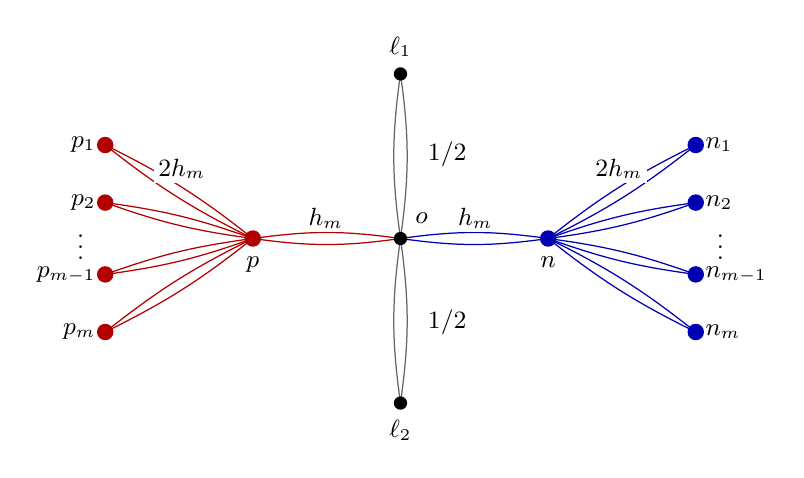
\begin{tikzpicture}[x=1.25cm,y=0.95cm,
  every node/.style={font=\small},
  vertex/.style={circle,fill=black,inner sep=1.7pt},
  hot/.style={circle,fill=red!70!black,inner sep=2.1pt},
  cold/.style={circle,fill=blue!70!black,inner sep=2.1pt},
  edge/.style={line width=0.45pt}]
\coordinate (o) at (0,0);
\coordinate (l1) at (0,2.2);
\coordinate (l2) at (0,-2.2);
\coordinate (p) at (-1.5,0);
\coordinate (n) at (1.5,0);
\foreach \A/\B/\col in {o/l1/black!60,o/l2/black!60,o/p/red!70!black,o/n/blue!70!black}{
  \draw[edge,\col] (\A) to[bend left=8] (\B);
  \draw[edge,\col] (\A) to[bend right=8] (\B);
}
\foreach \j/\y in {1/1.25,2/0.48,3/-0.48,4/-1.25}{
  \coordinate (p\j) at (-3.0,\y);
  \coordinate (n\j) at (3.0,\y);
  \draw[edge,red!70!black] (p) to[bend left=6] (p\j);
  \draw[edge,red!70!black] (p) to[bend right=6] (p\j);
  \draw[edge,blue!70!black] (n) to[bend left=6] (n\j);
  \draw[edge,blue!70!black] (n) to[bend right=6] (n\j);
  \node[hot] at (p\j) {};
  \node[cold] at (n\j) {};
}
\node[vertex,label=above right:$o$] at (o) {};
\node[hot,label=below:$p$] at (p) {};
\node[cold,label=below:$n$] at (n) {};
\node[vertex,label=above:$\ell_1$] at (l1) {};
\node[vertex,label=below:$\ell_2$] at (l2) {};
\node[left] at (p1) {$p_1$};
\node[left] at (p2) {$p_2$};
\node[left] at (p3) {$p_{m-1}$};
\node[left] at (p4) {$p_m$};
\node[right] at (n1) {$n_1$};
\node[right] at (n2) {$n_2$};
\node[right] at (n3) {$n_{m-1}$};
\node[right] at (n4) {$n_m$};
\node at (-3.25,0) {$\vdots$};
\node at (3.25,0) {$\vdots$};
\node[fill=white,inner sep=1.5pt] at (-0.76,0.27) {$h_m$};
\node[fill=white,inner sep=1.5pt] at (0.76,0.27) {$h_m$};
\node[fill=white,inner sep=1.5pt] at (-2.22,0.93) {$2h_m$};
\node[fill=white,inner sep=1.5pt] at (2.22,0.93) {$2h_m$};
\node[right] at (0.18,1.12) {$1/2$};
\node[right] at (0.18,-1.12) {$1/2$};
\end{tikzpicture}

  \caption{Schematic of \(\Gamma_m\), with representative fan edges shown.
  There are \(m\) distinct tips at each fan hub, and every displayed edge
  has two equal-length copies. The two long pairs have length \(1/2\)
  per copy, the stems length \(h_m\), and the fan edges length \(2h_m\).
  The drawing is not to metric scale. Red and blue tips are respectively
  all global maxima and all global minima of the mode in
  Section~\ref{sec:extrema}; both long pairs have zero mode value.
  Deleting one copy of each edge gives the comparison tree \(T_m\).}
  \label{fig:graph}
\end{figure}

The parameter choice ensures
\begin{equation}\label{eq:length-bounds}
  0<h\leq\frac{\arctan(1/2)}{\pi}<\frac16,\qquad
  b=2h<\frac13,\qquad h+b=3h<\frac12.
\end{equation}
In the source construction the unlengthened fan leaf has length
\(\pi^{-1}\arctan(\cot(\pi h)/m)\), which equals \(h\) at our choice
of \(h\). Thus \(b=2h\) corresponds to lengthening each fan leaf by
\(h\). The proof below orders the resulting spectrum directly;
it does not require an unspecified small perturbation.

\section{The first positive tree eigenvalue}\label{sec:tree-spectrum}

We first retain the full leaf-permutation decomposition.
At either hub, write the \(m\) leaf functions as their common mean
plus \(m-1\) zero-sum components. Continuity forces the zero-sum
components to vanish at the hub, while their endpoint fluxes cancel
in the sum. These components therefore give \(m-1\)
Dirichlet--Neumann interval sectors of length \(b\) per fan.
Their wave numbers are
\begin{equation}\label{eq:leaf-sectors}
  \frac{(2r+1)\pi}{2b}=\frac{(2r+1)\pi}{4h},
  \qquad r=0,1,2,\ldots.
\end{equation}
Their first wave number exceeds \(\pi\), since \(h<1/6<1/4\).
The complementary invariant subspace has identical functions on
all leaves at each hub. This is a decomposition of the whole
operator, rather than an imposed equal-leaf ansatz.

\subsection{A single fan with a Dirichlet root}

Put a Dirichlet condition at the root \(o\) of one fan, and use
coordinates \(x\in[0,h]\) from root to hub and \(y\in[0,b]\)
from hub to a leaf tip. At a positive wave number \(t\), its
equal-leaf mode has the form
\[
  w_s(x)=S\sin(tx),\qquad
  w_j(y)=C\cos(t(b-y)).
\]
Continuity and Kirchhoff flux at the hub give
\begin{equation}\label{eq:fan-matching}
  C\cos(tb)=S\sin(th),\qquad
  mC\sin(tb)=S\cos(th).
\end{equation}
The characteristic equation, written without division by a
trigonometric factor, is
\begin{equation}\label{eq:fan-char}
  F(t):=\cos(th)\cos(tb)-m\sin(th)\sin(tb)=0.
\end{equation}
For \(0<t\leq\pi\), both \(th\) and \(tb\) belong to \((0,\pi/2)\).
The function \(m\tan(th)\tan(tb)\) is strictly increasing from zero
and at \(t=\pi\) equals
\[
  m\frac{1}{\sqrt m}\frac{2/\sqrt m}{1-1/m}
  =\frac{2m}{m-1}>1.
\]
Hence the fan has exactly one Dirichlet-root wave number below \(\pi\).
Writing \(z=\tan(th)\) and using \(b=2h\), its equation becomes
\[
  \frac{2mz^2}{1-z^2}=1,\qquad z^2=\frac{1}{2m+1}.
\]
The root is precisely \(t=k\), is simple, and satisfies \(k<\pi\).
Together with \eqref{eq:leaf-sectors}, this also shows that the full
rooted fan has no lower positive eigenvalue. The two rooted long arms
are Dirichlet--Neumann intervals of length \(1/2\), whose first wave
number is \(\pi\).

\subsection{Excluding lower full-tree modes and proving simplicity}

Suppose \(0<t<k\) and let \(c\) denote an eigenfunction's value at \(o\).
There are no leaf zero-sum modes in this range. On each long arm the
outgoing derivative at \(o\) is
\[
  ct\tan(t/2).
\]
On each equal-leaf fan, solving the two hub equations gives outgoing
root derivative
\[
  ct\,
  \frac{\tan(th)+m\tan(tb)}
       {1-m\tan(th)\tan(tb)}.
\]
Both coefficients multiplying \(c\) are strictly positive throughout
\(0<t<k\). Thus the central Kirchhoff condition is impossible when
\(c\ne0\). When \(c=0\), all four root-Dirichlet branches are
invertible in this range, so the function vanishes. This excludes
every positive eigenvalue below \(k^2\).

At \(t=k\), allow a nonzero root value and write the stem as
\(c\cos(kx)+S\sin(kx)\). The exact hub equations are
\begin{align}
  C\cos(kb)-S\sin(kh)&=c\cos(kh),\label{eq:inhom1}\\
  mC\sin(kb)-S\cos(kh)&=-c\sin(kh).\label{eq:inhom2}
\end{align}
Because \(F(k)=0\), the left side of \eqref{eq:inhom2} is
\(\cot(kh)\) times the left side of \eqref{eq:inhom1}.
Compatibility therefore requires
\[
  -c\sin(kh)=\frac{c\cos^2(kh)}{\sin(kh)},
\]
and hence \(c=0\). No singular expression is used outside its stated
range, where \(\sin(kh)>0\).

The long arms consequently vanish, since \(k<\pi\).
Each fan has one remaining amplitude \(S_+\) or \(S_-\), and the
central flux equation is
\[
  k(S_++S_-)=0.
\]
It leaves exactly one nonzero eigendirection. We have proved
\begin{equation}\label{eq:tree-eigenvalue}
  \mu_2(\T)=k^2<\pi^2,\qquad
  \dim\ker(H_{\T}-k^2)=1.
\end{equation}
This proof includes all sectors and orders the lowest positive
eigenvalue in the full standard domain.

\section{Uniform doubling and the full operator}

For clarity we state the complete decomposition behind the known
doubling operation. It is essential here to retain the additional
Dirichlet sectors.

\begin{lemma}\label{lem:doubling}
Let \(T\) be a finite compact standard-Kirchhoff metric graph and
let \(G\) replace every edge \(e\) of length \(L_e\) by two equal
parallel copies. Then
\begin{equation}\label{eq:unitary}
  H_G\ \simeq\ H_T\;\oplus\!
  \bigoplus_{e\in E(T)}\HDD(0,L_e).
\end{equation}
The direct sum includes all eigenvalues and their multiplicities.
\end{lemma}

\begin{proof}
Align the coordinates of each pair and define
\[
  g_e=\frac{f_{e,1}+f_{e,2}}{\sqrt2},\qquad
  q_e=\frac{f_{e,1}-f_{e,2}}{\sqrt2}.
\]
This transformation is unitary in the edgewise \(L^2\) spaces.
Continuity of \(f\) makes \(q_e\) zero at both endpoints.
All incident endpoint values of \(g\) are equal, being \(\sqrt2\)
times the common physical vertex value.
The sum of the two copied-edge derivatives at a vertex is
\(\sqrt2\) times the corresponding derivative of \(g_e\); the
\(q_e\) derivatives cancel. Since every original edge is doubled,
the full vertex equation reduces exactly to the Kirchhoff equation
for \(g\) on \(T\).

Conversely, any \(g\in D(H_T)\) and independent
\(q_e\in H^2(0,L_e)\cap H^1_0(0,L_e)\) reconstruct
\(f_{e,1}=(g_e+q_e)/\sqrt2\) and
\(f_{e,2}=(g_e-q_e)/\sqrt2\) in \(D(H_G)\).
The differential actions commute with this transformation.
This two-sided domain map proves \eqref{eq:unitary}.
\end{proof}

Each added interval has eigenvalues \((r\pi/L_e)^2\),
\(r=1,2,\ldots\). For \(\T\), all \(L_e\leq1/2\).
Thus every added eigenvalue is at least \(4\pi^2\), strictly above
the simple tree eigenvalue \(k^2<\pi^2\). Equation
\eqref{eq:unitary} therefore gives
\begin{equation}\label{eq:doubled-eigenvalue}
  \mu_2(\G)=k^2,\qquad
  \dim\ker(H_{\G}-k^2)=1.
\end{equation}
Its eigenfunction has equal profiles on paired copies.
Uniform doubling is used at all vertices; doubling only a selection
of edges would in general change the symmetric vertex equations
and would not justify this conclusion.

\section{Every extremum and every metric distance}\label{sec:extrema}

Choose the tree eigenfunction with \(S_+=1\) and \(S_-=-1\).
The long arms are identically zero. On the positive stem and on
each positive fan edge its profiles are
\begin{equation}\label{eq:profiles}
  \psi_s(x)=\sin(kx),\qquad
  \psi_j(y)=C_m\cos(k(2h-y)),\qquad
  C_m=\frac{\sin\theta}{\cos(2\theta)}
      =\frac{\sqrt{m+1}}{\sqrt2\,m}>0.
\end{equation}
The negative fan has the opposite profiles.
Indeed,
\[
  \sin\theta=\frac{1}{\sqrt{2m+2}},\qquad
  \cos(2\theta)=\frac{m}{m+1},\qquad
  \sin(2\theta)=\frac{\sqrt{2m+1}}{m+1},
\]
which verify both equations in \eqref{eq:fan-matching}.
Use these same unnormalized profiles on both copies in \(\G\).

Because \(0<\theta<\pi/4\), the positive stem is strictly increasing
away from \(o\), and every positive fan edge is strictly increasing
up to its tip: its derivative is positive on \(0\leq y<2h\).
The hub value is \(C_m\cos(2\theta)<C_m\).
The negative fan is strictly decreasing in the same orientations.
All other points have values strictly between the global extremes.
Consequently
\begin{equation}\label{eq:complete-M}
  \M(\G)=\{p_1,\ldots,p_m,n_1,\ldots,n_m\}.
\end{equation}
In particular, the equal values on the long arms do not create
global extrema, and none of the copied edge interiors is omitted.

On \(\T\), tips at the same hub are distance \(4h\) apart, and tips
at opposite hubs are distance \(6h\) apart. The long tips
\(\ell_1,\ell_2\) are distance one apart; any long tip and any fan
tip are distance \(1/2+3h<1\) apart.
A geodesic in a finite tree extends, if necessary, to a path between
leaves. These leaf distances therefore prove the full continuum
diameter \(\diam\T=1\).

Folding every parallel pair onto its tree edge defines a map
\(P:\G\to\T\) that does not increase path lengths. Hence
\[
  \dist_{\T}(Px,Py)\leq\dist_{\G}(x,y).
\]
For vertices, the tree geodesic lifts to \(\G\), giving equality.
The same is true for points that project to distinct original
edges: the unique tree path lifts with the prescribed copy at
either end. Points on a single common copy also have their tree
distance. Only points in opposite copies of the \emph{same}
original edge need a separate estimate.

For that last case, use coordinates \(s,t\in[0,L]\) on aligned
copies. A route through either endpoint has length \(s+t\) or
\(2L-s-t\), respectively. There is no external path between
these endpoints avoiding the pair, since deleting the original
edge disconnects the tree. Thus their exact distance is
\begin{equation}\label{eq:opposite-distance}
  \min\{s+t,\,2L-s-t\}\leq L\leq\frac12.
\end{equation}
These cases exhaust all pairs of points in the doubled graph.
Every distance is at most one, and the two long tips still realize
one. Vertex distances, including all distances in
\eqref{eq:complete-M}, are unchanged by doubling. Therefore
\[
  \diam\G=1,\qquad \diam\M(\G)=6h.
\]

Each copied edge belongs to the two-edge cycle formed with its
mate. Thus \(\G\) has no bridge and every point lies on a cycle.
Finally, \(\arctan t<t\) for \(t>0\) and
\eqref{eq:epsilon-choice} imply
\[
  6h_m
  =\frac{6}{\pi}\arctan(m^{-1/2})
  <\frac{6}{\pi\sqrt m}
  \leq\varepsilon.
\]
The chosen \(m\) is finite for every positive \(\varepsilon\).
This completes the proof of Theorem~\ref{thm:main}.

\section{Network diffusion and the scope of the construction}

For a uniform physical diffusivity \(D>0\), the heat equation on
these networks is
\[
  \partial_t u=-D H_\Gamma u.
\]
Kirchhoff flux conserves the integral of \(u\), and the constant
mode is equilibrium. If the initial temperature has a nonzero
projection onto the simple first positive mode, its slowest
nonconstant component is
\[
  A e^{-D\mu_2t}\psi_2.
\]
For that component the entire hottest/coldest set has the spatial
diameter calculated above. A sufficiently large constant background
makes this sign-changing temperature deviation compatible with
positive absolute temperature. The statement about \(\M\) is
exactly about the eigenmode; at finite times higher modes may
split the symmetry ties.

Taking the diameter as one length unit, Theorem~\ref{thm:main}
excludes a positive universal lower bound on the fraction of
network diameter spanned by the complete extrema set of a simple
slowest mode, even when all edges are cyclic. Restoring a length
scale \(L_0\) multiplies all distances by \(L_0\) and sends the
eigenvalue to \(k_m^2/L_0^2\).
Thus \(D\mu_2\) has units of inverse time.

The construction has \(4m+8\) edges after doubling and total length
\begin{equation}\label{eq:total-length}
  |\Gamma_m|=2+4h_m+8mh_m.
\end{equation}
The degree of each fan hub is \(2m+2\).
Both total length and hub degree grow along the family.
Articulation vertices remain. We therefore establish the precise
no-bridge conjecture, without adding fixed-volume, uniformly
bounded-degree, vertex-biconnected, Euclidean-domain, or experimental
conclusions.

All spectral, extremal, and metric assertions in the proof are
exact for every integer \(m\geq4\). The accompanying reproducibility
files provide the analytic argument and diagnostic programs based
on full endpoint matching, exact algebraic identities, and
optimization over interior edge-pair coordinates. Floating-point
roots, ranks, and metric samples are diagnostics rather than
interval certificates, and are not used to prove the quantified
existence statement.

\section*{Use of generative AI tools}

OpenAI Codex was used for literature screening, development of the
construction and analytic arguments, implementation of diagnostic
calculations, internal checking, and drafting the text and the
diagram. These uses include AI-generated scientific text and proof
development throughout the article. Internal AI checks are not
external peer review and may share errors; literature coverage is
bounded. Human scientific review and author approval of this draft
remain pending.

\section*{Data and code availability}

The reproducibility supplement contains the explicit construction,
the exact analytic argument, input records, diagnostic code, and
environment and regeneration instructions. It contains no
experimental data. The proof does not depend on a numerical
enclosure or spatial truncation.

\bibliographystyle{plainnat}
\bibliography{references}
\end{document}
